    \section{Análise da Concorrência}

No processo de desenvolvimento deste projeto e na análise do mercado correspondente, foram identificada e examinadas     diversas aplicações com potencial concorrencial em relação ao \textit{GameLocker}. Nesse contexto, torna-se imprescindível a avaliação minuciosa destes concorrentes, visando à compreensão aprofundada de suas fraquezas e fortalezas. Simultaneamente, almeja-se a identificação das áreas nas quais a \textit{GameLocker} possui a oportunidade de se destacar perante esses competidores.

Ao apresentar a totalidade dos concorrentes devidamente elencados e detalhados no presente documento, emerge a identificação de dois competidores primordiais: os portais \textit{\gls{Alvanista}} e \textit{\gls{GGApp}}. Esta delimitação permite direcionar a análise de forma mais específica e concentrada, viabilizando uma investigação mais detalhada das estratégias e características que delineiam essas duas plataformas em relação à \textit{GameLocker}.

\subsection{Alvanista}

A plataforma \textit{\gls{Alvanista}} \cite{alvanista}, disponibilizada de forma gratuita, emerge como uma ferramenta de relevância incontestável. Ela se destaca ao proporcionar recursos essenciais, abrangendo a catalogação da biblioteca de jogos, a monitorização contínua do progresso individual do usuário, a viabilização de trocas de recomendações entre os participantes, a facilitação da imersão em comunidades de interesse específico e a facilitação da interconexão entre jogadores. A Figura \ref{Alvanista}, apresentada no formato próprio para ambiente online, proporciona uma representação visual da interface da plataforma. Esta imagem não apenas destaca a sua estrutura de maneira vívida, mas também evidencia a plenitude das funcionalidades incorporadas.

\begin{figure}[H]
	\centering
	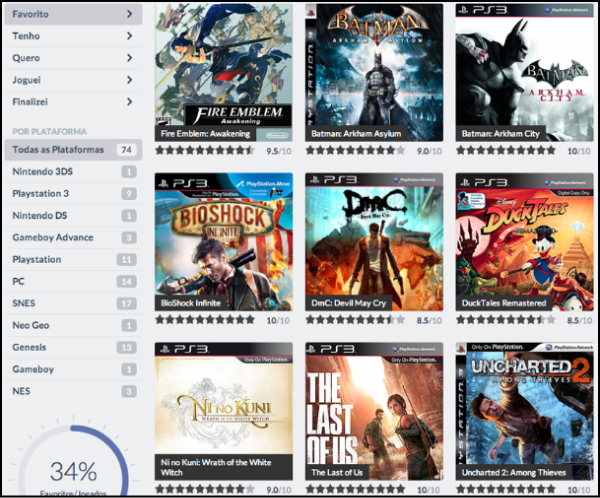
\includegraphics[scale=0.6]{./imagens/introducao/alvanista.png}
	\caption{Plataforma Alvanista}
	\label{Alvanista}
	Fonte: \cite{alvanista}
\end{figure}

A usabilidade deficiente torna a navegação pelo site complicada e confusa, dificultando a busca por informações e recursos importantes. Além da ausência de uma arena de jogos, a privação dos usuários da oportunidade de participarem de competições e desafios com outros jogadores. Tal ausência pode resultar em uma experiência menos emocionante e desestimular os usuários que buscam um ambiente competitivo.

\subsection{GG App}

O aplicativo móvel e a plataforma online \textit{\gls{GGApp}} \cite{ggapp}, como evidenciado na Figura \ref{ggapp}, apresentam-se como um conjunto integral, proporcionando uma gama diversificada de recursos destinados tanto à gestão eficaz de jogos quanto à promoção de interações entre os jogadores. Concebido com um propósito preciso, ele visa aprimorar a experiência dos jogadores, facilitando não apenas o controle das suas coleções de jogos, mas também incentivando a exploração de novos títulos, o estabelecimento de conexões com amigos e a imersão em comunidades virtuais.

\begin{figure}[H]
	\centering
	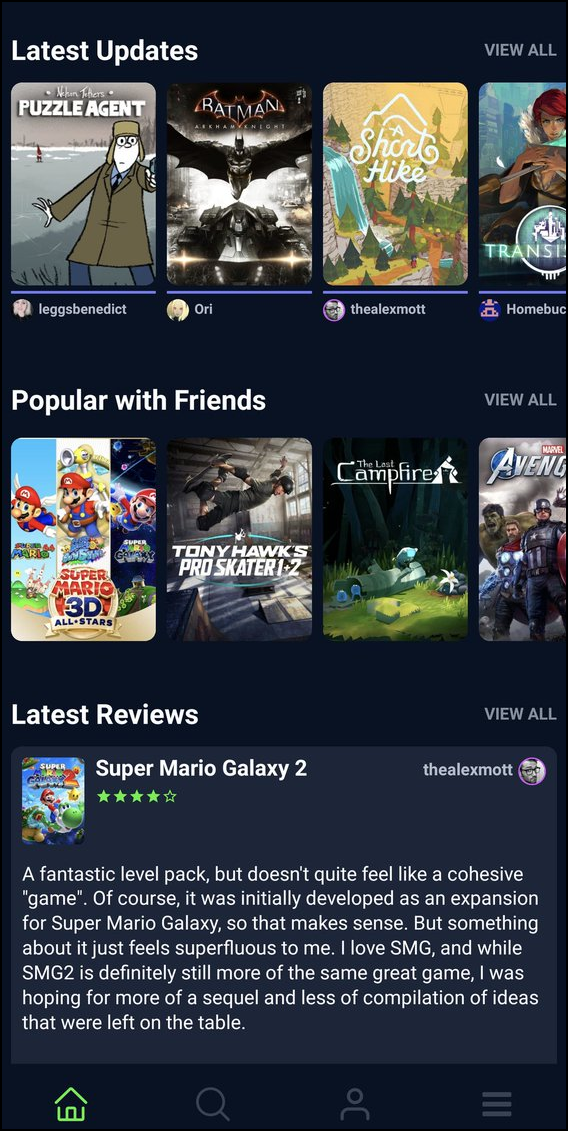
\includegraphics[scale=0.35]{./imagens/introducao/ggapp.png}
	\caption{Plataforma GG App}
	\label{ggapp}
	Fonte: \cite{ggapp}
\end{figure}

Uma arena de jogos oferece uma plataforma que possibilita aos jogadores interagirem entre si, seja por meio de chat ou em partidas competitivas. A ausência dessa funcionalidade pode resultar em uma experiência menos atraente para os usuários, com potencial para diminuição do engajamento, redução da interação social e dificuldades na medição de habilidades e promoção de jogos. A presença dessa arena promove uma atmosfera competitiva e socialmente interativa, encorajando a participação ativa dos usuários e incentivando melhorias contínuas nos jogos. Ademais, a falta dessa característica pode afetar negativamente a atratividade da plataforma perante outros serviços similares que fornecem esse recurso, afastando potenciais usuários em busca de uma experiência mais completa e imersiva.

\subsection{Comparação de Aplicativos Concorrentes}

Por meio das análises efetuadas, pôde-se constatar que tanto o \textit{\gls{Alvanista}} quanto o \textit{\gls{GGApp}} apresentam atributos que possibilitam a administração eficaz e a disseminação de avaliações relacionadas a jogos, além de propiciarem um ambiente propício para a interatividade entre seus usuários. No entanto, é relevante ressaltar que esses aplicativos não colocam uma ênfase significativa na criação de um espaço dedicado à competição direta entre os jogadores, conforme destacado no Quadro \ref{quadroConcorrente}.

\begin{quadro}[thb]
\centering
\ABNTEXfontereduzida
\caption{Comparação de Aplicativos Concorrentes}

\begin{tabular}{|l|c|c|c|}
\hline
\thead{Funcionalidades} & \thead{GameLocker} & 
\thead{Alvanista} & \thead{GG APP} \\
\hline
Usabilidade & X &  & X \
\\\hline
Gestão de jogos & X & X & X \
\\\hline
Avaliação de jogos & X & X & X \
\\\hline
Interação Social & X & X & X \
\\\hline
Arena de Jogos & X &  &  \
\\\hline
\end{tabular}
\label{quadroConcorrente}
\fonte{Autores}
\end{quadro}

No contexto das funcionalidades identificadas, torna-se evidente a preponderância das ferramentas destinadas à gestão e à comunicação, com ambas as plataformas fomentando a troca de análises críticas e opiniões acerca dos jogos. Essa ênfase demonstra a orientação compartilhada entre os concorrentes em direção a um ambiente colaborativo e informativo, onde os jogadores podem engajar-se em discussões enriquecedoras.

Entretanto, a distinção reside na ausência de um espaço especialmente dedicado à competição entre os usuários, algo que poderia acrescentar uma dimensão adicional à experiência oferecida. Tal ênfase, como identificada no Quadro \ref{quadroConcorrente}, é uma característica potencialmente diferenciadora que a \textit{GameLocker} pode explorar para se posicionar de forma distintiva no mercado, ao cativar um público que busca um ambiente não apenas para intercâmbio de informações, mas também para a competição saudável e a busca por reconhecimento no cenário dos jogos.